\normalfont\normalsize
\chapter{Introduction}

\begin{quote} 
{\itshape \small
``A network of possibly low-size and low-complex devices denoted as nodes that can sense the environment and
communicate the information gathered from the monitored field (e.g. an area or volume) through wireless links; the data
is forwarded, possibily via multiple hops relaying, to a sink (sometimes denoted as controller or monitor) that can
use it locally, or is connected to other networks (e.g. the Internet) through a gateway. The nodes can be stationary
or moving. They can be aware of their location or not. They can be homogenous or not.''} as quoted from \cite{Chong2003}.
\end{quote}

The domain of Wireless Sensor and Actuator Networks (WS\&ANs) is an emergent multi-disciplinary field, because its
applications intertwine with a lot of other domains, such as medicine, biology, meteorology, different types of 
engineering. Whether it's for an irrigation system, package monitor, pulse monitor or weather station, 
wireless sensor networks have gained a serious footing in applications that need advanced sensor systems.

They were first designed for military applications, where one can imagine deployment is infinitely simpler without wires, 
one needs only to position the sensors and turn them on, while redeployment can mean just moving them around. As things evolved,
now we can expect to integrate this technology with just about any relevant field where gathering more data helps the system make
more intelligent decisions. 

\begin{figure}[ht]
 \begin{center}
  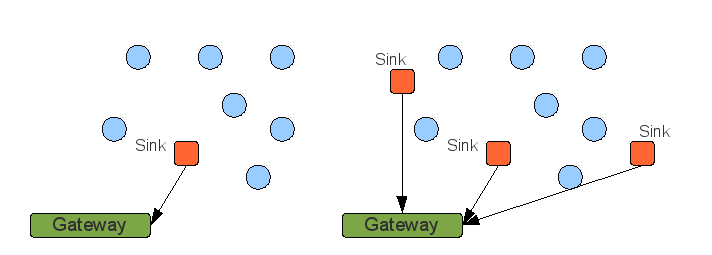
\includegraphics[scale=0.6]{wsan/wsansink.png}
 \end{center}
\caption{\small \itshape{A single-sink wireless sensor network (left), and multi-sink version (right). The gateway is connected to an 
external network, possibly the Internet}}

\end{figure}

Taking into consideration data flow, there are several types of WSNs: single-hop/single-sink, that have a star-like topology and
a single gateway, multi-hop / multi-sink, single-hop / multi-sink and multi-hop / single-sink. Single sink refers to the direction
in which sensor data flows, that is from source (sensor nodes) to a data sink (a gateway connecting the wireless sensor network
to a different type of network, which can be the Internet). Throughout this study we will consider single-sink networks, single-hop
or multi-hop. This type of network can be extended to include WS\&AN networks, by including actuator capabilities on the nodes. A single
sink for sensor data remains, but now data can flow in different directions, the nodes that have actuators can be commanded either by 
themselves, or by a neighbouring node, from the services running on the gateway or from the outside (via the gateway). We will
use WSN and WS\&AN terms intermittently in the study, as some properties are easily generalized.


There are several features a WSN can have: 
\begin{itemize}
\item \textit{Self-organization} - Refers to the emergence of global behaviour of a network from high-level rules on individual rules
on the nodes. As WSNs become more and more popular, the desire would be to minimize human intervention, to have the network 
organize itself. Also, a WSN with self-organization will be adaptable (it will be able to react to changes in the environment),
robustness (it will have the capability to repair damage to itself - self-healing), scalable (the WSN will work just as well
with a lot more nodes). \cite{Bett2005}
\item \textit{Self-healing} - Gives the network the possibility to recover from failure of individual nodes, to continue to 
offer the same services, as well as maintain network integrity by rerouting around failed nodes.
\item \textit{Energy efficiency} - Dictates every aspect of a WSN. Consumption has to be kept low in a WSN in order to
keep network lifetime to a maximum, either by minimizing radio communication or data processing or balacing it with 
energy harvesting.
\item \textit{Connectivity} - A network has to have to have sufficient connection and alternate routes between nodes, such that each node can
communicate with every other node even if one or more nodes have failed.
\item \textit{Low-Complexity} - Result of the fact that nodes must be small and minimal processing is needed. In WSNs, not a lot of processing power
in needed, as tasks that are required of the nodes are rather uncomplicated. Furthermore, lower complexity may mean smaller size, which is 
a desired feature.
\item \textit{Low-Cost} - In order to be a viable alternative to wired sensor systems, WSNs must offer low maintenance cost as well as low node cost.
The cheaper the nodes, the more can be integrated into a WSN with the same price, the greater the advantage over wired networks. Adding a new node 
to a WSN costs exactly as much as one node, no secondary expenses are needed.
\item \textit{Size of nodes} - Has to kept small in order to be able to integrate them well into the environment they will
interact with. The ultimate goal here is to build ``smart dust'', top-of-the-finger (or even smaller) that can act as basic nodes
in a WSN.
\end{itemize}





